\documentclass[a4paper]{article}

% Pacotes para o português.
\usepackage[brazilian]{babel}
\usepackage[utf8]{inputenc}
\usepackage[T1]{fontenc}

\usepackage{datetime}
\usepackage{graphicx}

% Usado nos pedaços de código.
\usepackage{listings}
\lstset{language=C,
	basicstyle=\small\sffamily,
	numbers=left,
	numberstyle=\tiny,
	frame=tb,
	columns=fullflexible,
	showstringspaces=false,
	captionpos=b}
\renewcommand\lstlistingname{Código}

\newcommand{\HRule}{\rule{\linewidth}{0.5mm}}

\begin{document}

\begin{titlepage}
\begin{center}	

% Topo 1.
\textsc{\Large UNIVERSIDADE DE SÃO PAULO\\
	INSTITUTO DE CIÊNCIAS MATEMÁTICAS E DE COMPUTAÇÃO}\\[0.7cm]

% Topo 2.
\textsc{\Large SSC0143}\\[0.2cm]
\textsc{\Large Programação Concorrente - Turma B}\\[0.5cm]

% Título.
\HRule \\[0.4cm]
{ \huge \bfseries Palíndromos}\\[0.4cm]
\HRule \\[0.4cm]
\textsc{Professor Dr. Julio Estrella}\\[1.5cm]

% Grupo
\begin{minipage}{0.4\textwidth}
\begin{flushleft} \large
\emph{Grupo 06:}\\
Bruno Junqueira Adami\\
Lucas Junqueira Adami\\
Lucas Lobosque\\
\end{flushleft}
\end{minipage}
\begin{minipage}{0.4\textwidth}
\begin{flushright} \large
\emph{Números USP:}\\
6878762\\
6792496\\
6792645\\
\end{flushright}
\end{minipage}

\vfill

% Rodapé.
{\large \today}
	
\end{center}
\end{titlepage}

\section{Introdução}
\indent \indent O problema proposto é o de devesenvolver versões de um programa paralelo para realizar as tarefas de determinar a ocorrência de palíndromos em dois textos especificados. Além disso, no texto maior, uma vez encontrado o palíndromo, é preciso determinar se a soma dos números correspondentes ao mapeamento do código ASCII de cada caracter da palavra é um número primo. Para calcular se o número é primo, o algoritmo de crivo de Erastótenes deve ser utilizado. As bibliotecas OpenMP e OpenMPI foram utilizadas para realizar o trabalho paralelo.\\
\indent Para realizar o desenvolvimento da proposta, o projeto foi separado em três partes:
\begin{itemize}
	\item Execução do algoritmo do crivo.
	\item Leitura dos arquivos de entrada.
	\item Cálculo dos palíndromos.
\end{itemize}
\indent \indent Todas as execuções citadas no documento, responsáveis pela geração dos gráficos, foram executados no cluster disponível.

\section{O projeto OpenMP}
\indent \indent Neste projeto, a paralelização do código foi feita nos loops do programa através das chamadas dos macros da biblioteca. O programa segue um fluxo contínuo e possui blocos de código executados em paralelo. Inicialmente, o cálculo do crivo é feito. Após esse passo, os arquivos são lidos e as palavras lidas são entregues ao verificador de palíndromos. A execução do programa e seus resultados apresentam-se na figura~\ref{graph-omp}.
\begin{figure}[float=p]
	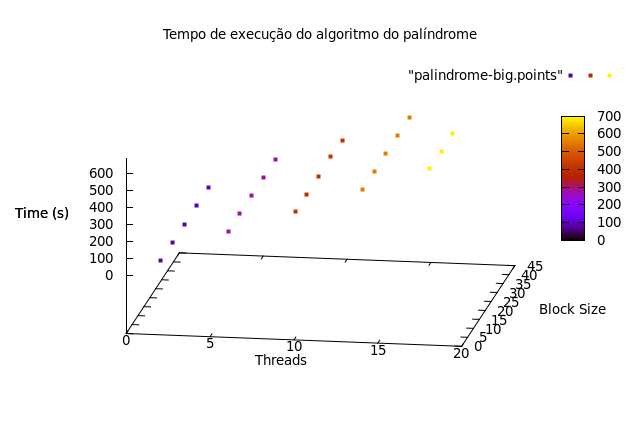
\includegraphics[scale=0.5]{graph-omp}
	\caption{Resultados da execução do projeto MPI}
	\label{graph-omp}
\end{figure}

\subsection{Execução do parser}
\indent \indent TODO.

\subsection{Cálculo dos palíndromos}
\indent \indent O algoritmo de cálculo dos palíndromos é simples. Sua complexidade é \begin{math}O(n)\end{math}, pois baseia-se em apenas um loop para verificar a palavra. Além disso, ele já soma os valores ASCII dos caracteres para responder se a soma total é um número primo. Para a paralelização do algoritmo, o macro citado no código~\ref{code-macro1} foi utilizado. Neste passo, a decomposição de dados foi utilizada. O vetor que contém a palavra é dividido em sessões que serão computadas pela OpenMP através da chamada do macro. Cada partição executa o loop com suas iterações correspondentes em paralelo.
\begin{lstlisting}[caption=Macro que paraleliza o algoritmo do palíndromo, label=code-macro1]
#pragma omp parallel for num_threads(PALINDROME_N_THREADS) 
	schedule(dynamic, PALINDROME_BLOCK_SIZE) reduction(+:sum) 
	reduction(&&:palindrome)
\end{lstlisting}
\indent \indent As definições PALINDROME\_N\_THREADS e PALINDROME\_BLOCK\_SIZE são passadas ao programa através do arquivo makefile. A primeira diz quantas threads serão utilizadas na paralelização do loop. A segunda, quantas iterações cada thread irá realizar. A palavra dynamic define que não haverá uma ordem na distribuição das iterações para os loops. Neste macro também estão definidas as reduções da soma para verificar a primalidade e da validade do palíndromo.\\
\indent Alguns testes foram aplicados isoladamente do resto do sistema para testar a performance do algoritmo e suas diferentes configurações. Uma leitura cega foi feita dos dois arquivos de entrada e os resultados obtidos estão presentes na figura~\ref{graph-palindrome-small} e na figura~\ref{graph-palindrome-big}.
\begin{figure}[float=p]
	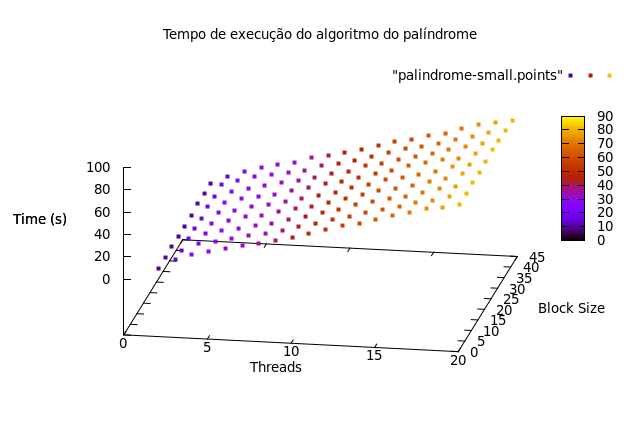
\includegraphics[scale=0.5]{graph-palindrome-small}
	\caption{Resultados do algoritmo do palíndromo para o arquivo menor}
	\label{graph-palindrome-small}
\end{figure}
\begin{figure}[float=p]
	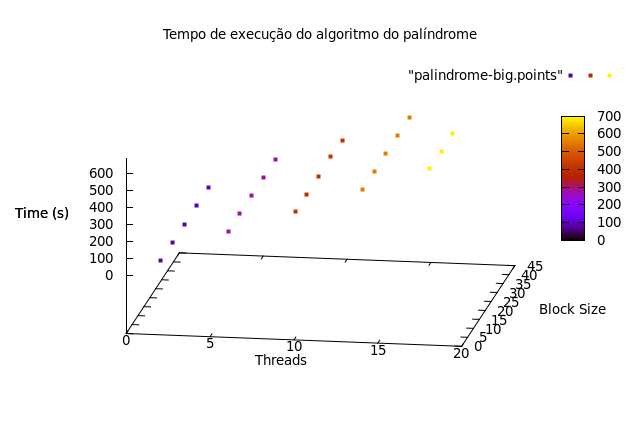
\includegraphics[scale=0.5]{graph-palindrome-big}
	\caption{Resultados do algoritmo do palíndromo para o arquivo maior}
	\label{graph-palindrome-big}
\end{figure}
Os valores do números de threads e o tamanho do bloco que cada thread executa foram baseados em valores estimados. Um cálculo do tamanho médio das palavras provenientes da leitura cega apontou que para o arquivo menor, essa média valia 40 e para o maior, 4.

\subsection{Cálculo do crivo}
\indent \indent O crivo de Eratóstenes é um algoritmo e um método simples e prático para encontrar números primos até um certo valor limite. Segundo a tradição, foi criado pelo matemático grego Eratóstenes (c. 285-194 a.C.), o terceiro bibliotecário-chefe da biblioteca de Alexandria.\\
\indent O algoritmo se baseia em marcar os múltiplos dos primos encontrados até agora. Os números não marcados serão os números primos. Deve-se iterar do número 2 em diante até a raíz do maior número que se deseja calcular. A complexidade do algoritmo é \begin{math}O(n\log(\log n))\end{math}.\\
\indent Na implementação deste trabalho os números pares são ignorados para otimizar um pouco o método. A função isPrime testa se o número par é primo ou não. No caso, apenas o 2 será. Se o número for ímpar, esta função irá checar o vetor de marcação dos múltiplos.\\
\indent A decomposição utilizada foi a de dados, pois foi paralelizada a demarcação dos mútiplos dos números primos, onde cada thread fica responsável por um trecho do vetor dos múltiplos. Para isso usou-se o código~\ref{code-macro2}, que separa o for em vários blocos, o número de blocos é determinado pelo macro SIEVE\_N\_THREADS. A implementação em OpenMP paraleliza a parte que faz a marcação dos múltiplos do primo encontrado. No fim para saber se o número é primo ou não, basta apenas checar o vetor de marcação dos múltiplos.
\begin{lstlisting}[caption=Macro que paraleliza o algoritmo do palíndromo, label=code-macro2]
#pragma omp parallel for num_threads(SIEVE_N_THREADS)
\end{lstlisting}
\indent \indent Testes de performance foram aplicados isoladamente do resto do programa. Os resultados obtidos encontram-se na figura~\ref{graph-sieve-omp}.
\begin{figure}[float=p]
	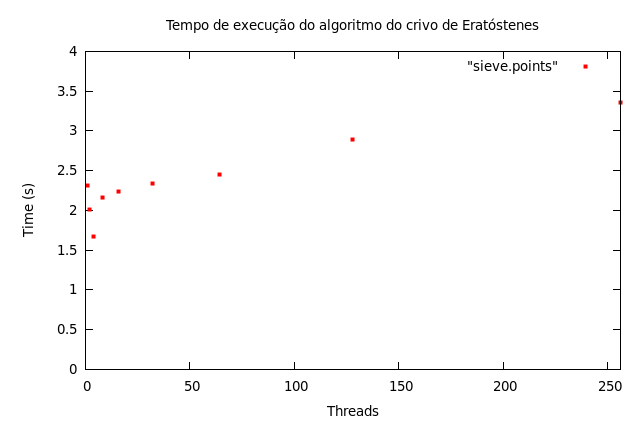
\includegraphics[scale=0.5]{graph-sieve-omp}
	\caption{Tempos de execução do crivo usando OpenMP}
	\label{graph-sieve-omp}
\end{figure}

\section{O projeto MPI}
\indent \indent O projeto MPI foi desenvolvido seguindo a estrutura da figura~\ref{pic-mpi}. Todos os processos do programa têm suas chamadas principais executadas no início do programa. Existem três tipos de processos:
\begin{itemize}
	\item Processos mestres principais.
	\item Processos mestres secundários.
	\item Processos escravos.
\end{itemize}
\begin{figure}[float=p]
	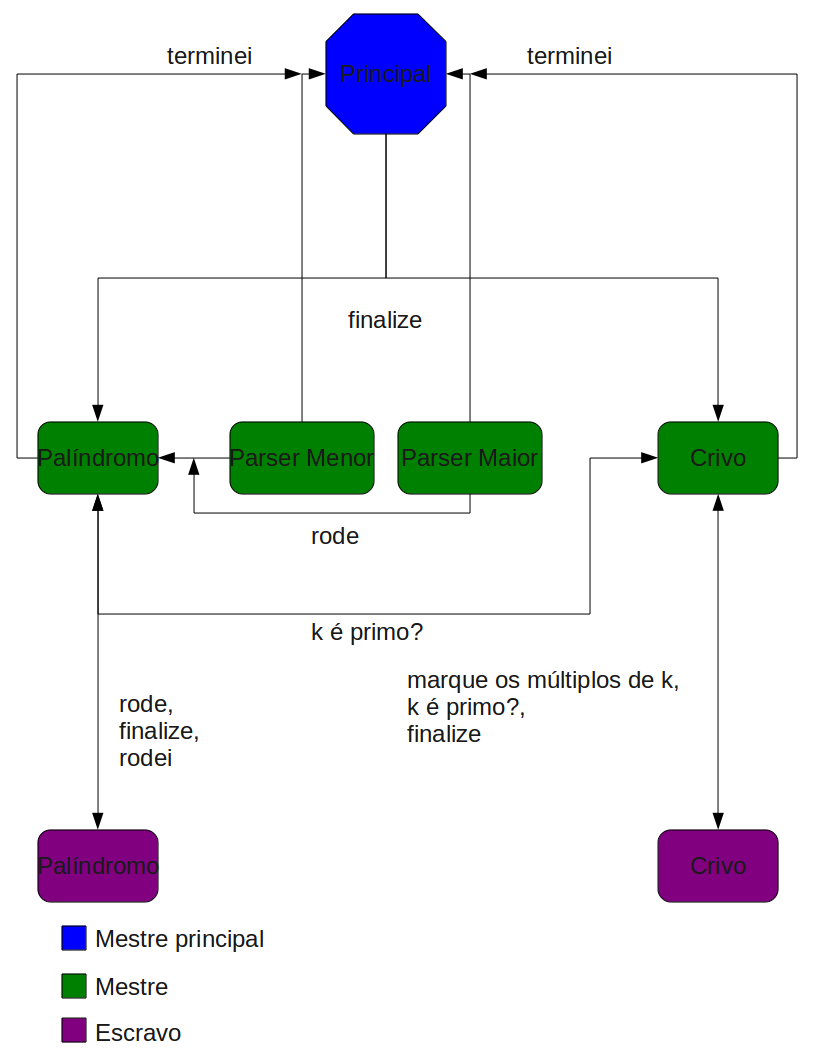
\includegraphics[scale=0.5]{pic-mpi}
	\caption{A estrutura do projeto MPI}
	\label{pic-mpi}
\end{figure}
\indent \indent Há somente um processo mestre principal. O mestre principal é responsável por controlar os processos do segundo tipo, os processos mestres secundários. Ele envia mensagens de finalização para esses processos e recebe informações de término ao final da execução deles. Neste projeto, todo o sistema foi testado em conjunto. Várias configurações de números de escravos foram utilizadas. Os resultado obtidos encontram-se na figura~\ref{graph-mpi}.
\begin{figure}[float=p]
	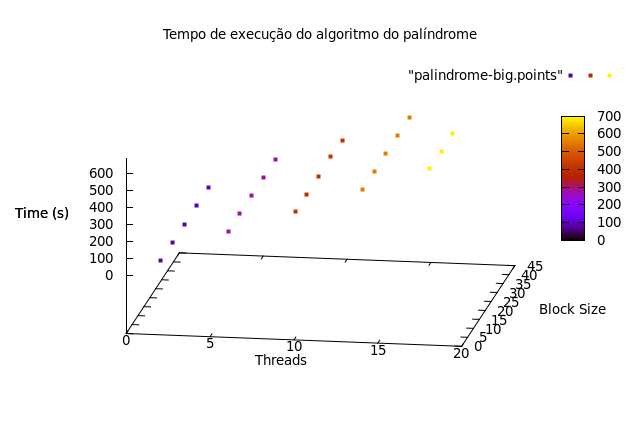
\includegraphics[scale=0.5]{graph-mpi}
	\caption{Resultados da execução do projeto MPI}
	\label{graph-mpi}
\end{figure}

\subsection{Execução do parser}
\indent \indent TODO.

\subsection{Cálculo dos palíndromos}
\indent \indent O algoritmo para o cálculo é o mesmo utilizado para o projeto OpenMP. Há um processo mestre que coordena os processos escravos. Ao receber uma palavra, o processo mestre envia a mensagem ao próximo escravo da fila (uma file round-robin) e o escravo executa o algoritmo do palíndromo, enviando ao mestre o resultado. Aqui, a decomposição pode ser vista como uma decomposição pseudo-especulativa. Na verdade, cada requisição pode ser executada paralelamente, independentemente de qualquer fator, funcionando como filas paralelas de execução de trabalho. A tomada de decisão, que é característica dessa decomposição não existe. O mestre apenas tem que saber qual o próximo escravo a receber uma palavra.

\subsection{Cálculo do crivo}
\indent \indent O algoritmo para o cálculo é análogo para o projeto OpenMP. O cálculo aqui também paraleliza a marcação dos mútiplos dos primos. O processo meste itera os números de 2 até a raiz do maior número e requisita ao processos escravos que demarquem os múltiplos dos primos. Para encontrar se um número é primo, o processo mestre faz uma requisição ao escravo que contém o intervalo do número requisitado. O escravo então responde ao processo mestre que responde ao processo que fez a pergunta se o número é primo ou não. A decomposição é a de dados, pelas mesmas razões citadas no projeto OpenMP.\\
\indent Assim como anteriormente, testes de performance foram aplicados isoladamente do resto do programa. Os tempos obtidos encontram-se na figura~\ref{graph-sieve-mpi}.
\begin{figure}[float=p]
	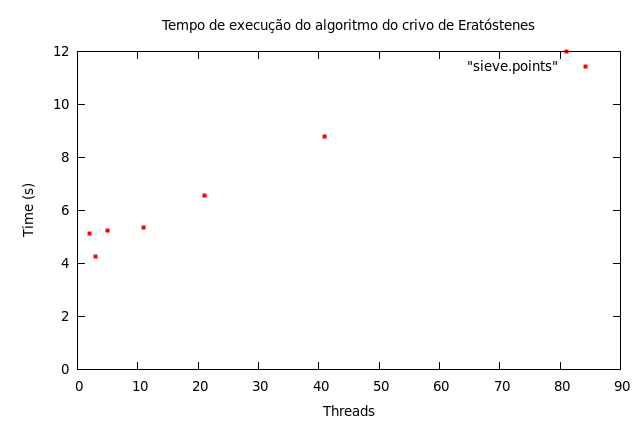
\includegraphics[scale=0.5]{graph-sieve-mpi}
	\caption{Tempos de execução do crivo usando MPI}
	\label{graph-sieve-mpi}
\end{figure}

\newpage
\begin{thebibliography}{99}
	\bibitem[OpenMP]{mp1}http://bisqwit.iki.fi/story/howto/openmp/
	\bibitem[OpenMP]{mp2}http://openmp.org/wp/
	\bibitem[Gnuplot]{gnuplot}http://www.duke.edu/~hpgavin/gnuplot.html
	\bibitem[Crivo de Eratóstenes]{crivo1} http://en.wikipedia.org/wiki/Sieve\_of\_Eratosthenes
	\bibitem[Crivo de Eratóstenes]{crivo2} http://www.algorithmist.com/index.php/Prime\_Sieve\_of\_Eratosthenes
	\bibitem[MPI]{mpi1} http://www.slac.stanford.edu/comp/unix/farm/mpi.html
	\bibitem[MPI]{mpi2} http://www.eecis.udel.edu/\~{}saunders/courses/372/01f/manual/manual.html
\end{thebibliography}
\end{document}
